\documentclass{article}
\usepackage{bm,sectsty,fancyhdr,multicol,lastpage}
\usepackage{amsmath,enumitem,tabularx,textcomp,nccmath,amssymb}
\usepackage{listings} % Insert bullet points
\usepackage[a4paper,left=1cm,right=1cm,top=2cm,bottom=2cm,headsep=0.5cm]{geometry}
\usepackage{xcolor} % Format color in code cells
\usepackage{titlesec} % Format title section
\usepackage{graphicx} % Embed images
\usepackage[document]{ragged2e} % Fix uneven spacing caused in multi col mode

% Define Colors
\definecolor{codegreen}{rgb}{0,0.6,0}
\definecolor{codegray}{rgb}{0.5,0.5,0.5}
\definecolor{codeorange}{rgb}{1,0.49,0}
\definecolor{backcolour}{rgb}{0.95,0.95,0.96}
\lstdefinestyle{mystyle}{
    backgroundcolor=\color{backcolour},
    commentstyle=\color{codegray},
    keywordstyle=\color{codeorange},
    numberstyle=\tiny\color{codegray},
    stringstyle=\color{codegreen},
    %basicstyle=\ttfamily\footnotesize,
    basicstyle=\tiny,
    breakatwhitespace=false,
    breaklines=true,
    captionpos=b,
    keepspaces=true,
    numbers=left,
    numbersep=5pt,
    showspaces=false,
    showstringspaces=false,
    showtabs=false,
    tabsize=2,
    xleftmargin=0pt,
    language=SQL,
    label={lst:code},
    mathescape=true,
    gobble=12
}
\lstset{style=mystyle}

% Header and Footer
\pagestyle{fancy}
\fancyhf{}
\fancyhead[L]{SQL Cheatsheet}
\fancyfoot[R]{Riten Patel}
\fancyfoot[L]{\LaTeX}
\fancyfoot[C]{\thepage\ of \pageref{LastPage}}
\renewcommand{\headrulewidth}{1.4pt}
\renewcommand{\footrulewidth}{1.4pt}

% Configurations
\sectionfont{\large}
\setlength{\columnsep}{0.5cm}
\setlength{\columnseprule}{1.4pt}
\setlength{\parindent}{0pt}
\setlength{\parskip}{-6pt}
\newcolumntype{Y}{>{\centering\arraybackslash}X}
\setlist[itemize]{nolistsep,left=0pt}
\graphicspath{{./images/}}
\tolerance=9999
\emergencystretch=10pt
\hyphenpenalty=10000
\exhyphenpenalty=100

\begin{document}
\begin{multicols*}{2}
    \raggedcolumns

    % Basic Commands
    \titleformat{\section}
        {\normalfont\fontfamily{phv}\fontsize{10}{0}\bfseries}{\thesection}{1em}{}
    \section{Basic Commands}
    \renewcommand\labelitemi{{\boldmath$\cdot$}}
    \begin{itemize}[noitemsep]
        \item CREATE TABLE: Creates a table
        \item INSERT: Inserts a row (or set of rows) into a given table
        \item UPDATE: Modifies already-existing data 
        \item DELETE: Removes a row (or groupe of rows)
        \item SELECT: Selects certain columns from a table
        \item GROUP BY: Groups rows having contents of a column
        \item WHERE: Filter \textbf{before} any grouping is applied
        \item HAVING: Filter \textbf{after} any grouping is applied
        \item ORDER BY: Sorts results by column(s)
        \item DISTINCT: Returns only distinct values
        \item UNION: Combines results from multiple tables
        \item DATE\_TRUNC(\emph{month}, \emph{timestamp}): extract month from timestamp
    \end{itemize}

    % Joins
    \titleformat{\section}
        {\normalfont\fontfamily{phv}\fontsize{10}{0}\bfseries}{\thesection}{1em}{}
    \section{Joins}
    \renewcommand\labelitemi{{\boldmath$\cdot$}}
    \begin{itemize}[noitemsep]
        \item OUTER JOIN: Combine and preserve all rows
        \item LEFT JOIN: Combine and preserve rows from left table
        \item RIGHT JOIN: Combine and preserve rows from right table
        \item JOIN: Combine and preserve rows from both tables \\
        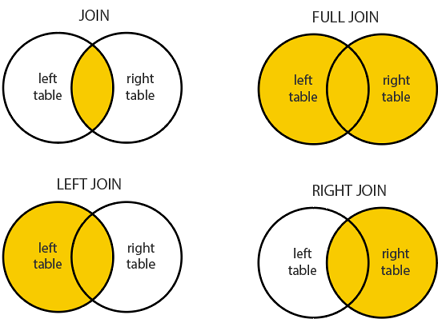
\includegraphics[width=\linewidth]{sql_joins}
        \begin{lstlisting}
            SELECT 
                COUNT(DISTINCT u.user_id)
            FROM 
                users u
                JOIN posts p ON u.user_id = p.user_id
        \end{lstlisting} 
    \end{itemize}

    % Common Table Expressions and Subqueries
    \titleformat{\section}
        {\normalfont\fontfamily{phv}\fontsize{10}{0}\bfseries}{\thesection}{1em}{}
    \section{Common Table Expressions (CTEs) and Subqueries}
    \renewcommand\labelitemi{{\boldmath$\cdot$}}
    \begin{itemize}[noitemsep]
        \item CTEs: Define a table and allow it to be referenced later using an alias  
        (i.e distribution of posts by users)
        \begin{lstlisting}
            WITH user_post_count AS (
                SELECT
                    users.user_id,
                    COUNT(post_id) AS num_posts
                FROM users
                LEFT JOIN posts on users.user_id = posts.user_id 
                GROUP BY 1
            )

            SELECT num_posts, COUNT(*) as num_users
            FROM user_post_count 
            GROUP BY 1
        \end{lstlisting}
        \item Subqueries: are inline in the query itself and must have a unique alias
        \begin{lstlisting}
            SELECT num_posts, COUNT(*) as num_users
            FROM
                (
                SELECT users.user_id,
                    COUNT(post_id) as num_posts
                FROM users
                    LEFT JOIN posts on users.user_id = posts.user_id 
                GROUP BY 1
                ) u
        \end{lstlisting}
    \end{itemize}

    % Window Functions
    \titleformat{\section}
        {\normalfont\fontfamily{phv}\fontsize{10}{0}\bfseries}{\thesection}{1em}{}
    \section{Window Functions}
    \renewcommand\labelitemi{{\boldmath$\cdot$}}
    \begin{itemize}[noitemsep]
        \item Window Functions: Performs a calculation across a set of rows. This 
        can be done by an aggregation function. But unlike regular aggregate 
        functions, a window function \textbf{does not} cause rows to become grouped 
        into a single output row - the rows retain their separate identities. i.e.. 
        \begin{lstlisting}
            SELECT 
                first_name, last_name, department_id,
                ROUND(AVG(salary) OVER (PARTITION BY department_id)) as avg_dep_salary
            FROM 
                employees;
        \end{lstlisting}
        \item PARTITION BY: like GROUP BY, separates rows into partitions
        \item ORDER BY: order in which rows are processed
        \item ROWS BETWEEN (start, end): which rows to process 
        \begin{itemize}
            \item \emph{start} PRECEDING AND \emph{end} FOLLOWING
            \item UNBOUNDED PRECEDING AND \emph{end} FOLLOWING
            \item CURRENT ROW
        \end{itemize}
        \item LAG(\emph{column}, \emph{offset}): Access previous rows per defined offset value
        \item LEAD(\emph{column}, \emph{offset}): Access following rows per defined offset value
        \item RANK(): specify rank each row by a defined column
        \item DENSE\_RANK(): specify a unique rank number, unlike RANK() if we have 
        duplicate values, the duplicate has the same rank but the rank does not 
        give any gap for the values. i.e..
        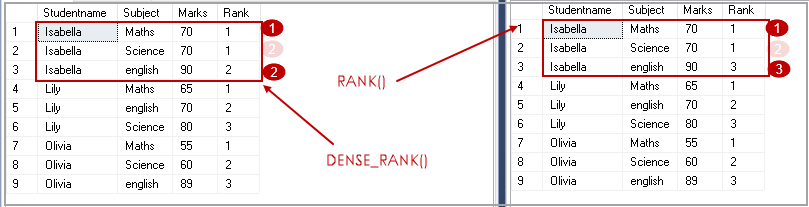
\includegraphics[width=\linewidth]{rank_vs_denserank}
        \item ROW\_NUMBER(): get a unique sequential number for each row even 
        if they have duplicates. i.e..
        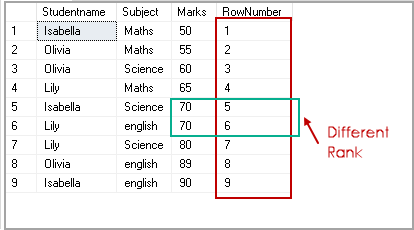
\includegraphics[width=\linewidth]{row_number}
        \item CUME\_DIST(): finds cumulative distance (0,1]
        \item PERCENT\_RANK(): finds percentile [0,1]
    \end{itemize}

     % Databases and Systems
     \titleformat{\section}
     {\normalfont\fontfamily{phv}\fontsize{10}{0}\bfseries}{\thesection}{1em}{}
     \section{Databases and Systems}
    \renewcommand\labelitemi{{\boldmath$\cdot$}}
    \begin{itemize}[noitemsep]
        \item Primary Key: field uniquely identifying each row
        \item Foreign Key: field linking two related tables
        \item Normalization: process of separating data to prevent redundancy
        \item Denormalization: optimization technique to keep redudndant data to 
        prevent expensive join operations
        \item Database view: like a normal table but with no schema. Advantages include:
        simplification of workflow by aggregating tables, dynamically computed meaning 
        less memory overhead, limited table exposure
        \item Properties of Distributed Databases
        \begin{itemize}
            \item CAP Theorem for assessing properties of a distributed db \\
            \textbf{C}onsistency: all clients using db see same data \\
            \textbf{A}vailability: system is always available \\
            \textbf{P}artition tolerance: system functions
            even if node communication is lost/delayed
            \item ACID framework for measuring correctness and completeness of a relational db transaction \\
            \textbf{A}tomicity: entire transaction occurs as a whole or it doesn't occur at all \\
            \textbf{C}onsistency: ensures db is consistent before/after a transacation is completed \\
            \textbf{I}solation: transaction occurs in isolation so that 
            multiple transactions occur independently without interference \\
            \textbf{D}urability: once a transaction is completed, the db is properly updated
            \item BASE framework for NoSQL databases, similar to ACID \\
            \textbf{Ba}sically Available: There will always be a response to any request, but 
            the data may be inconsistent and inaccurate \\
            \textbf{S}oft State: systems's state may change over time, even without input \\
            \textbf{E}ventual Consistency: data will converge to a consistent state, no guarantees of when
        \end{itemize}
        \item Scaling Databases
        \begin{itemize}
            \item Vertical scaling: add CPU and RAM to existing machines. 
            Easy to administer but expensive as certain machines may be close to their physical limits
            \item Horizontal scaling: add more machines (nodes) to the resource pool. 
            Much cheaper and better fault tolerance but difficult to administer (data consistency between nodes)
            \item Sharding: Split rows across nodes in a cluster
        \end{itemize}
        \item Relational Databases: store data in a table-based structure
        \item NoSQL Databases: store data in forms other than 
        table-based \\
        - Document databases - allow complex, nested, varied schemas inside of it (i.e. MongoDB, Elasticsearch) \\
        - Graph databases - data stored by relationships to other data records (i.e. Neo4J)
        \item MapReduce: parallel big data processing framework 
        \begin{itemize}
            \item 1. Split: splits input data and distributes across nodes
            \item 2. Map: take input data and output $<$key, value$>$ pairs 
            \item 3. Shuffle: move $<$key, value$>$ pairs with same key to same node
            \item 4. Reduce: aggregate $<$key, value$>$ pairs into final output
        \end{itemize}
        \item Spark: another parallel big data processing framework. Faster than MapReduce as 
        it uses RAM for computation enabling faster in-memory performance but higher running costs
    \end{itemize}

\end{multicols*}
\end{document}